\section{Estrutura} \label{Secao Estrutura}

O suporte ou rolo, como é comumente chamado pelos ciclistas, tem como papel transformar uma bicicleta normal em uma do tipo ergométrica, uma vez que este suporte irá levantar a roda traseira ou as duas, dependendo do modelo, fazendo com que a bicicleta permaneça fixa no local em que se realiza a atividade física.  Existem atualmente no mercado, quatros tipos mais comuns de rolos de treinamento:
1.	Rolo de equilíbrio
2.	Rolo de treinamento de resistência magnética
3.	Rolo de treinamento com resistência de fluidos
4.	Rolo de treinamento comum
Na figura \ref{fig:rolos} a seguir, podemos visualizar na seqüência, os quatros tipos:

\begin{figure}[h]
    \centering
    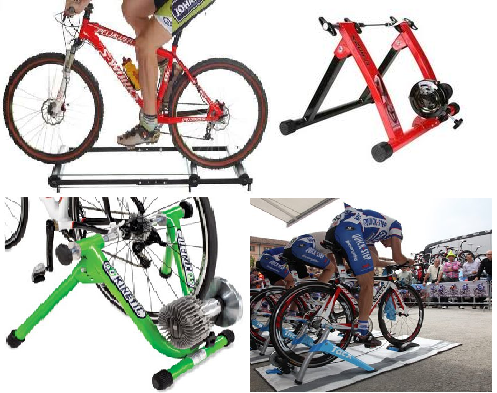
\includegraphics[width=0.8\textwidth]{figuras/rolos.png}
    \caption{Estrutura}
    \label{fig:rolos}
\end{figure}


Na presente divisão \ref{Secao Estrutura}  a estrutura baseada....na figura \ref{fig:awesome_image} ..... tendo como referencia \cite{shigley2011shigley}.

\begin{figure}[h]
    \centering
    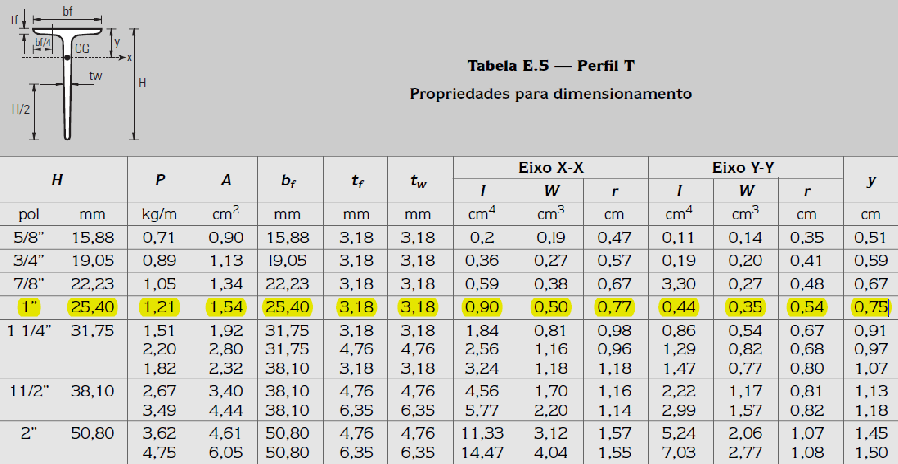
\includegraphics[width=0.8\textwidth]{figuras/perfil_t.png}
    \caption{Estrutura}
    \label{fig:awesome_image}
\end{figure}
